\chapter{KẾT QUẢ THỰC NGHIỆM}
\label{chap:results}

\section{Thiết lập}
\label{sec:setup}

Mọi số liệu dưới đây dùng ngưỡng IoU $\ge 0.5$. Tham số và lựa chọn phương pháp được chọn trên tập tune (198 ảnh); các bảng chính báo trên tập test (462 ảnh) và chỉ đo cho cấu hình đã chốt. Các nhóm khó (\code{blur}, \code{db}, \code{challenge}, \code{tilt}) chỉ có 12 ảnh ở tune và 28 ảnh ở test, nên một ảnh đổi kết quả làm tỉ lệ thay đổi $1/28\approx 0.036$; chênh lệch nhỏ ở các nhóm này không nên đọc là xu hướng. Thời gian chạy (ms/ảnh) trong chương này đo trên một lần chạy một tiến trình, máy ít tải hơn so với các lần chạy ghi trong sổ thí nghiệm (khi đó nhiều tiến trình khác chạy cùng lúc, số tuyệt đối cao gấp khoảng ba lần); vì vậy chỉ nên so sánh tương đối giữa các dòng của cùng một bảng. Số đo lại trên máy ít tải được ghi ở mục ``Đo lại thời gian (máy ít tải)'', ngày 2026-11-11, trong sổ thí nghiệm \code{notes.md}; bảng trong báo cáo dùng đúng các số đó.

\section{Tiền xử lý: kích thước ảnh và bộ lọc nhiễu (E2)}
\label{sec:e2}

\textbf{Kích thước ảnh.} Ở giai đoạn đầu (tập tune, cấu hình định vị cũ), thử ba chiều rộng resize cho thấy ảnh càng lớn càng tốt (Bảng~\ref{tab:resize}); giữ 800.

\begin{table}[htbp]
\centering
\caption[Ảnh hưởng của chiều rộng resize (tune)]{Ảnh hưởng của chiều rộng resize (tune, $n=198$, cấu hình định vị giai đoạn đầu; nguồn: sổ thí nghiệm, mục Tiền xử lý).}
\label{tab:resize}
\small
\rowcolors{2}{white}{tablerowalt}
\arrayrulecolor{tableheader}
\begin{tabularx}{\textwidth}{lCCCC}
\hline
\rowcolor{tableheader} \tblhd{Chiều rộng} & \tblhd{P} & \tblhd{R} & \tblhd{F1} & \tblhd{R@5} \\
\hline
640 & 0.639 & 0.591 & 0.614 & 0.727 \\
720 (không đổi tỉ lệ) & 0.640 & 0.601 & 0.620 & 0.758 \\
\textbf{800 (chọn, phóng to)} & 0.647 & 0.621 & 0.634 & 0.778 \\
\hline
\end{tabularx}
\end{table}

\textbf{Bộ lọc nhiễu.} E2 chạy \code{localize\_edge} với bốn bộ lọc và cấu hình chốt của mục~\ref{sec:tuning}, trên cả tune và test (Bảng~\ref{tab:e2}). Bộ lọc được chọn chỉ theo F1 trên tune.

\begin{tabular}{llrrrrrr}
\toprule
Tập & Bộ lọc & $n$ & P & R & F1 & R@5 & ms/ảnh \\
\midrule
tune & \textbf{bilateral} & 198 & 0.775 & 0.747 & 0.761 & 0.828 & 132.5 \\
tune & gaussian & 198 & 0.630 & 0.601 & 0.615 & 0.682 & 95.0 \\
tune & median & 198 & 0.637 & 0.611 & 0.624 & 0.697 & 107.7 \\
tune & none & 198 & 0.598 & 0.571 & 0.584 & 0.657 & 97.4 \\
\midrule
test & \textbf{bilateral} & 462 & 0.729 & 0.682 & 0.705 & 0.792 & 111.1 \\
test & gaussian & 462 & 0.647 & 0.615 & 0.630 & 0.712 & 82.4 \\
test & median & 462 & 0.616 & 0.584 & 0.600 & 0.699 & 93.2 \\
test & none & 462 & 0.610 & 0.576 & 0.592 & 0.645 & 84.7 \\
\bottomrule
\end{tabular}


Bilateral cho F1 cao hơn rõ rệt trên cả hai tập: 0.761 so với 0.584--0.624 trên tune và 0.705 so với 0.592--0.630 trên test. Ba bộ lọc còn lại cho kết quả gần nhau, và trên test bộ lọc trung vị (0.600) chỉ nhỉnh hơn \code{none} (0.592) rất ít. Nguyên nhân có thể là bilateral làm mịn nhiễu và các chi tiết nền mà vẫn giữ cạnh nét ký tự, nên bản đồ cạnh Sobel ít ứng viên rác hơn (đây là giả thuyết, chưa kiểm tra riêng). Cái giá là thời gian: bilateral chậm hơn các bộ lọc khác khoảng 18--29 ms/ảnh trong lần đo này (111 ms so với 82--93 ms trên test). Chênh thời gian này đảo ngược so với lần đo khi máy đang tải (khi đó chênh giữa các bộ lọc gần như biến mất; xem mục đo lại trong \code{notes.md}), nên chênh thời gian giữa các bộ lọc nhạy với tải máy. Nên dùng bilateral cho các thí nghiệm sau.

\section{Hệ màu: độ tách biển khỏi nền (E1)}
\label{sec:e1}

Cách đo ở mục~\ref{sec:color}.

\begin{table}[htbp]
\centering
\caption[E1: độ tách biển / nền theo kênh màu (tune)]{E1: khoảng cách Bhattacharyya trung bình giữa histogram trong biển và ngoài biển, tune ($n=198$), xếp theo cột ALL. Trong ngoặc là độ lệch chuẩn giữa các ảnh. Nguồn: \code{e1\_color.csv}.}
\label{tab:e1}
\small
\rowcolors{2}{white}{tablerowalt}
\arrayrulecolor{tableheader}
\begin{tabularx}{\textwidth}{lCCCCCC}
\hline
\rowcolor{tableheader} \tblhd{Kênh} & \tblhd{base} & \tblhd{blur} & \tblhd{challenge} & \tblhd{db} & \tblhd{tilt} & \tblhd{ALL} \\
\hline
\textbf{b (Lab)} & 0.687 & 0.629 & 0.670 & 0.481 & 0.466 & \textbf{0.657} (0.130) \\
\textbf{H (HSV)} & 0.681 & 0.621 & 0.697 & 0.500 & 0.462 & \textbf{0.654} (0.141) \\
S (HSV) & 0.525 & 0.558 & 0.569 & 0.385 & 0.387 & 0.513 (0.135) \\
V (HSV) & 0.485 & 0.537 & 0.527 & 0.496 & 0.358 & 0.484 (0.121) \\
a (Lab) & 0.502 & 0.414 & 0.451 & 0.328 & 0.347 & 0.474 (0.129) \\
xám & 0.474 & 0.495 & 0.552 & 0.451 & 0.370 & 0.472 (0.106) \\
L (Lab) & 0.465 & 0.491 & 0.548 & 0.468 & 0.357 & 0.465 (0.112) \\
\hline
\end{tabularx}
\end{table}

\begin{figure}[htbp]
\centering
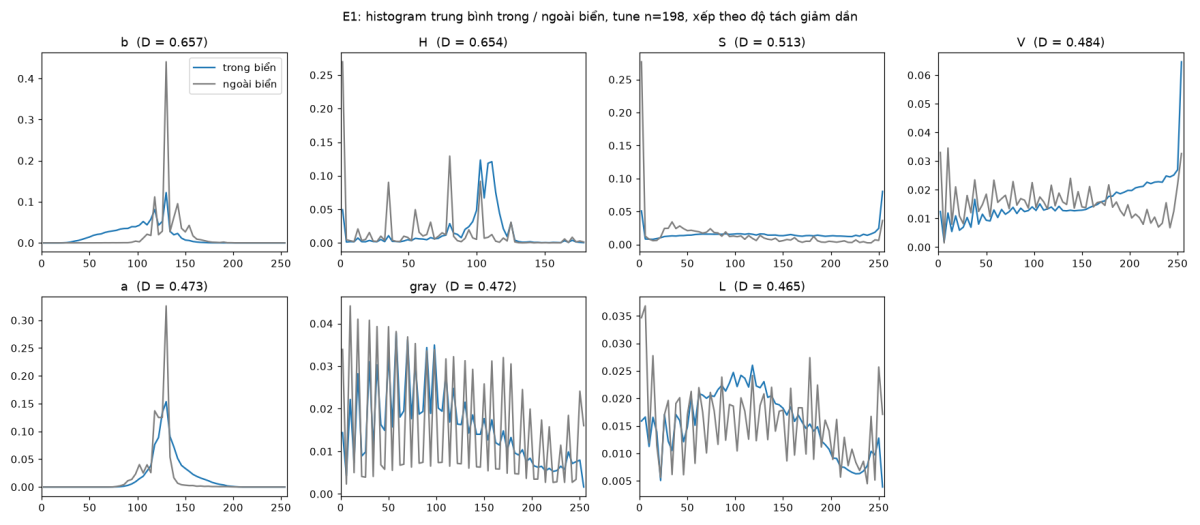
\includegraphics[width=\textwidth]{figures/e1_hist.png}
\caption[E1: histogram trung bình trong và ngoài biển]{E1: histogram trung bình trong biển (xanh) và ngoài biển (xám) của bảy kênh, tune $n=198$, xếp theo độ tách giảm dần.}
\label{fig:e1}
\end{figure}

\textbf{Nhận xét.}
\begin{itemize}
  \item \textbf{b và H tách tốt nhất} ($D\approx 0.65$), S đứng thứ ba (0.51); xám, L, V và a gần như hòa ($\approx 0.47$). Biển CCPD nền xanh dương: trong Lab màu xanh dương nằm ở phía $b<128$, trong HSV dồn vào khoảng $H\approx 100$--$120$ (Hình~\ref{fig:e1}), nên hai kênh này gom gọn vùng biển và lệch khỏi nền. Ảnh xám và L chỉ đo độ sáng, mà nền biển xanh đậm có độ sáng gần với thân xe và mặt đường.
  \item \textbf{Thứ hạng ổn định theo số bin:} đo lại với 32 và 128 bin, ba hạng đầu không đổi (b $\approx$ H $>$ S); bốn kênh cuối đổi chỗ cho nhau với chênh lệch dưới 0.02, coi như hòa.
  \item \textbf{Theo nhóm:} \code{db} và \code{tilt} tách kém nhất ở mọi kênh. Ở \code{db} biển tối hoặc chói làm màu mất bão hòa, nên V ($0.496$) gần bằng H ($0.500$); ở \code{tilt} bbox ngang của biển nghiêng ôm cả nền.
  \item Histogram H ngoài biển có đỉnh lớn ở 0: pixel xám hoặc trắng có $S\approx 0$ nên H không xác định và OpenCV gán 0. Răng cưa đều ở các kênh xám, L, V là do lượng tử hóa khi giải nén JPEG và đổi hệ màu, không làm đổi thứ hạng.
\end{itemize}

\textbf{Hệ quả và hạn chế.} Pipeline hiện định vị trên ảnh xám, kênh có độ tách gần thấp nhất. Một nguồn ứng viên theo màu (ví dụ tỉ lệ pixel có $H\in[95,135]$ và S đủ lớn) là hướng bổ sung tự nhiên cho khâu sinh ứng viên, đúng chỗ mà 21\% ảnh test không có ứng viên đúng trong top-5 (mục~\ref{sec:triage}); hướng này chưa được thử. Tuy nhiên kết luận này gắn với biển nền xanh của CCPD: biển Việt Nam nền trắng hoặc vàng sẽ không có lợi thế ở kênh H và b. Ngoài ra ``ngoài biển'' là toàn bộ phần ảnh còn lại, nên $D$ đo biển so với toàn cảnh chứ không phải so với vùng ngay sát biển, và histogram trong biển gồm cả ký tự trắng lẫn viền.

\section{Tinh chỉnh bước định vị trên tập tune}
\label{sec:tuning}

Cấu hình ban đầu (kernel close $17\times 3$, \code{fill\_ratio} tối thiểu 0.5, \code{edge\_density} tối thiểu 0.15) chỉ đạt Recall 0.348 trên tune. Quét từng tham số, mỗi lần đổi một hoặc hai tham số, cho thấy bước tăng lớn nhất là nới ngưỡng \code{fill\_ratio} và \code{edge\_density} (mặt nạ biển thật chỉ lấp khoảng 0.5 hình chữ nhật và mật độ cạnh khoảng 0.2), tiếp theo là chọn kernel close ngang rộng hơn (Bảng~\ref{tab:sweep}).

\begin{table}[htbp]
\centering
\caption[Một số dòng của đợt quét tham số định vị (tune)]{Một số dòng của đợt quét tham số định vị (tune, $n=198$, \code{localize\_edge}, top-1; \code{area\_ratio} $[0.002,0.10]$, chưa đa tỉ lệ). Nguồn: sổ thí nghiệm, mục Định vị.}
\label{tab:sweep}
\small
\rowcolors{2}{white}{tablerowalt}
\arrayrulecolor{tableheader}
\begin{tabularx}{\textwidth}{lCCCC}
\hline
\rowcolor{tableheader} \tblhd{Cấu hình} & \tblhd{P} & \tblhd{R} & \tblhd{F1} & \tblhd{R@5} \\
\hline
Mặc định cũ: close $[17,3]$, fill 0.5, dens 0.15 & 0.570 & 0.348 & 0.433 & 0.384 \\
fill 0.35, dens 0.10 (close $[17,3]$) & 0.545 & 0.515 & 0.530 & 0.682 \\
fill 0.35, dens 0.10 + close $[25,5]$ & 0.647 & 0.621 & 0.634 & 0.778 \\
fill 0.35, dens 0.10 + close $[21,5]$ & 0.672 & 0.641 & 0.656 & 0.783 \\
\textbf{close $[21,5]$, fill 0.40, dens 0.12 (chốt)} & \textbf{0.703} & \textbf{0.646} & \textbf{0.674} & \textbf{0.768} \\
\hline
\end{tabularx}
\end{table}

\textbf{Tinh chỉnh bộ lọc ứng viên (recall của ứng viên).} Sau đó chúng tôi nhận thấy biển thật thường bị bỏ sót vì vùng biển vỡ mảnh sau bước hình thái học, hoặc bị ứng viên nhỏ (logo, chữ) xếp trên. Tăng $k$ từ 5 lên 10 không đổi Recall, tức nút thắt nằm ở bộ lọc chứ không phải số ứng viên giữ lại. Top-1 sai thường là một vùng rất nhỏ (\code{area\_ratio} khoảng 0.002--0.003) trong khi biển thật có \code{area\_ratio} khoảng 0.015--0.05. Ba thay đổi được chọn trên tune: (i) thêm hai kernel close phụ và gộp bằng NMS, (ii) nâng cận dưới \code{area\_ratio} từ 0.002 lên 0.008 và cận trên từ 0.10 lên 0.16 theo phân bố bbox thật, (iii) nới \code{aspect} từ $[2,6]$ lên $[1.5,7]$ vì quad của vùng cạnh nghiêng hoặc dính viền dài/ngắn hơn biển thật. Bảng~\ref{tab:i10abl} cho thấy phần đóng góp của từng thay đổi trên tune; Bảng~\ref{tab:i10} so sánh trước và sau theo nhóm, đo trên test đúng một lần cho cấu hình chốt.

\begin{table}[htbp]
\centering
\caption[Tinh chỉnh bộ lọc ứng viên: đóng góp của từng thay đổi (tune)]{Tinh chỉnh bộ lọc ứng viên: đóng góp của từng thay đổi (tune, $n=198$, ALL, top-1). \code{cand\_recall} là Recall@5. Nguồn: sổ thí nghiệm, mục tinh chỉnh bộ lọc ứng viên.}
\label{tab:i10abl}
\small
\rowcolors{2}{white}{tablerowalt}
\arrayrulecolor{tableheader}
\begin{tabularx}{\textwidth}{lCCC}
\hline
\rowcolor{tableheader} \tblhd{Cấu hình} & \tblhd{\code{cand\_recall}} & \tblhd{Recall@1} & \tblhd{P} \\
\hline
Cũ (close $[21,5]$, aspect $[2,6]$, area $[0.002,0.10]$) & 0.768 & 0.646 & 0.703 \\
Chỉ thêm hai kernel close $[13,3]$, $[33,7]$ & 0.828 & 0.652 & 0.665 \\
Chỉ đổi area thành $[0.008,0.16]$ & 0.753 & 0.712 & 0.829 \\
Area $[0.008,0.16]$ + hai kernel thêm & 0.818 & 0.747 & 0.787 \\
\textbf{+ aspect $[1.5,7.0]$ (chốt)} & \textbf{0.828} & \textbf{0.747} & \textbf{0.775} \\
\hline
\end{tabularx}
\end{table}

\begin{table}[htbp]
\centering
\caption[Tinh chỉnh bộ lọc ứng viên: cấu hình cũ so với cấu hình chốt (test)]{Tinh chỉnh bộ lọc ứng viên: cấu hình cũ $\to$ cấu hình chốt, tập test ($n=462$), \code{localize\_edge} (chưa SVM). Nguồn: sổ thí nghiệm, mục tinh chỉnh bộ lọc ứng viên. Ở tune (ALL, $n=198$): \code{cand\_recall} $0.768\to 0.828$, Recall@1 $0.646\to 0.747$, P $0.703\to 0.775$.}
\label{tab:i10}
\small
\rowcolors{2}{white}{tablerowalt}
\arrayrulecolor{tableheader}
\begin{tabularx}{\textwidth}{lCCCC}
\hline
\rowcolor{tableheader} \tblhd{Nhóm} & \tblhd{$n$} & \tblhd{\code{cand\_recall}} & \tblhd{Recall@1} & \tblhd{P} \\
\hline
base & 350 & $0.729\to 0.874$ & $0.609\to 0.751$ & $0.644\to 0.771$ \\
blur & 28 & $0.500\to 0.643$ & $0.357\to 0.643$ & $0.400\to 0.750$ \\
challenge & 28 & $0.571\to 0.500$ & $0.429\to 0.464$ & $0.500\to 0.619$ \\
db & 28 & $0.464\to 0.429$ & $0.321\to 0.321$ & $0.409\to 0.409$ \\
tilt & 28 & $0.357\to 0.571$ & $0.286\to 0.429$ & $0.348\to 0.500$ \\
\hline
ALL & 462 & $0.667\to 0.792$ & $0.545\to 0.682$ & $0.593\to 0.729$ \\
\hline
\end{tabularx}
\end{table}

Trên test, Recall@1 tăng từ 0.545 lên 0.682 và \code{cand\_recall} từ 0.667 lên 0.792, tức cải thiện không chỉ do khớp tune. Phần lớn lợi ích nằm ở nhóm \code{base} (Recall@1 $0.609\to 0.751$). Hai nhóm \code{db} và \code{challenge} gần như không đổi hoặc giảm nhẹ \code{cand\_recall} (với $n=28$ chỉ là 1--2 ảnh). Cái giá là thời gian: số ứng viên trung bình mỗi ảnh gần như không đổi nhưng thời gian tăng khoảng 40--50\% do thêm hai lượt hình thái học và tính đặc trưng (tune $309\to 426$ ms/ảnh, test $269\to 396$ ms/ảnh, đo khi máy đang tải nên chỉ mang tính tương đối). Cận diện tích không phải trần cứng: trên test có 16/462 bbox thật có \code{area\_ratio} dưới 0.008 (nhỏ nhất 0.0032) và 1 bbox lớn hơn 0.16, nhưng bộ lọc xét diện tích \code{minAreaRect} của \emph{ứng viên} chứ không phải của bbox thật, và IoU $\ge 0.5$ cho phép ứng viên lớn hơn bbox thật. Phần triage (mục~\ref{sec:triage}) cho thấy chỉ 12/16 bbox nhỏ bị mất ở bước định vị; 4 ảnh còn lại không mất ở đó. Bbox lớn duy nhất (\code{tilt\_0022}, 0.182) cũng không bị loại mà là lỗi xếp hạng (\code{loc\_rank}).

\section{Định vị: so sánh \code{edge} và \code{edge\_svm} (E3)}
\label{sec:e3}

\textbf{Huấn luyện SVM.} Trên 792 patch của tune (198 dương, 594 âm), kiểm chứng chéo 5 fold cho accuracy $0.960\pm 0.006$, precision $0.922\pm 0.035$, recall $0.919\pm 0.041$, F1 $0.919\pm 0.013$ (trung bình $\pm$ độ lệch chuẩn giữa các fold). Con số này lạc quan vì chia theo patch (các patch của cùng một ảnh có thể rơi vào cả train lẫn validation) và vì mẫu âm ngẫu nhiên khá dễ; độ chính xác định vị thực tế thấp hơn nhiều (bên dưới).

{\sloppy \textbf{Kết quả.} E3 dùng bộ lọc bilateral (chọn ở E2). Phương pháp được chọn theo F1 ALL trên tune: \code{edge\_svm} (F1 0.817, so với 0.761 của \code{edge}). Bảng~\ref{tab:e3} và Hình~\ref{fig:e3} cho kết quả trên test.\par}

\begin{table}[htbp]
\centering
\caption[E3: định vị theo nhóm (test)]{E3: định vị theo nhóm, tập test, bộ lọc bilateral. Nguồn: \code{e3\_localization.csv}.}
\label{tab:e3}
\small
\rowcolors{2}{white}{tablerowalt}
\arrayrulecolor{tableheader}
\begin{tabularx}{\textwidth}{llCCCCCCC}
\hline
\rowcolor{tableheader} \tblhd{Phương pháp} & \tblhd{Nhóm} & \tblhd{$n$} & \tblhd{P} & \tblhd{R} & \tblhd{F1} & \tblhd{R@1} & \tblhd{R@3} & \tblhd{R@5} \\
\hline
edge & base & 350 & 0.771 & 0.751 & 0.761 & 0.751 & 0.871 & 0.874 \\
edge & blur & 28 & 0.750 & 0.643 & 0.692 & 0.643 & 0.643 & 0.643 \\
edge & challenge & 28 & 0.619 & 0.464 & 0.531 & 0.464 & 0.500 & 0.500 \\
edge & db & 28 & 0.409 & 0.321 & 0.360 & 0.321 & 0.429 & 0.429 \\
edge & tilt & 28 & 0.500 & 0.429 & 0.462 & 0.429 & 0.571 & 0.571 \\
edge & ALL & 462 & 0.729 & 0.682 & 0.705 & 0.682 & 0.790 & 0.792 \\
\hline
edge\_svm & base & 350 & 0.856 & 0.834 & 0.845 & 0.834 & 0.874 & 0.874 \\
edge\_svm & blur & 28 & 0.667 & 0.571 & 0.615 & 0.571 & 0.643 & 0.643 \\
edge\_svm & challenge & 28 & 0.667 & 0.500 & 0.571 & 0.500 & 0.500 & 0.500 \\
edge\_svm & db & 28 & 0.500 & 0.393 & 0.440 & 0.393 & 0.429 & 0.429 \\
edge\_svm & tilt & 28 & 0.583 & 0.500 & 0.538 & 0.500 & 0.571 & 0.571 \\
edge\_svm & ALL & 462 & 0.803 & 0.751 & 0.776 & 0.751 & 0.792 & 0.792 \\
\hline
\end{tabularx}
\end{table}


\begin{figure}[htbp]
\centering
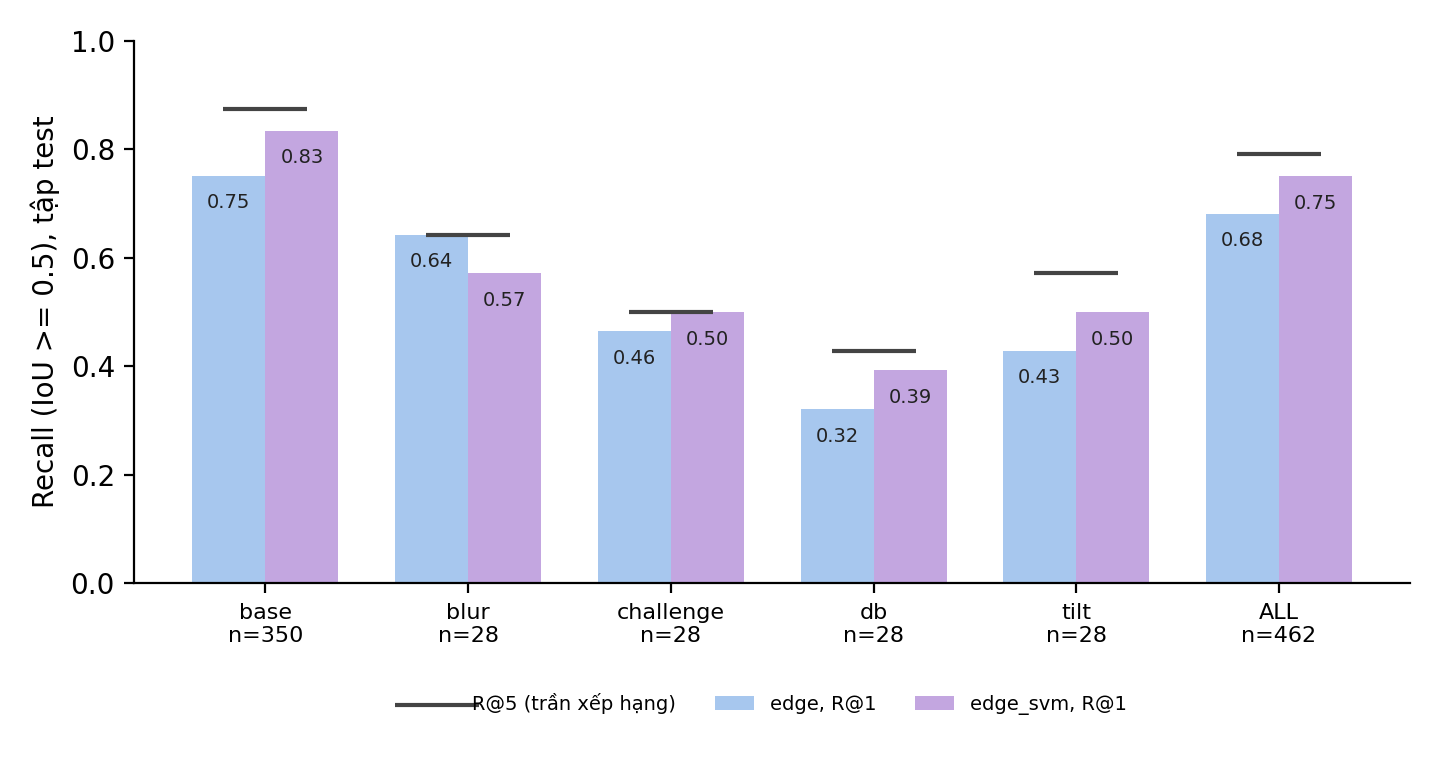
\includegraphics[width=0.85\textwidth]{figures/e3_subset_r1.png}
\caption[Recall@1 của edge và edge\_svm theo nhóm (test)]{Recall@1 của \code{edge} và \code{edge\_svm} theo nhóm (test). Vạch đen là Recall@5, trần mà bước xếp hạng không vượt qua được. Nguồn: \code{e3\_localization.csv}.}
\label{fig:e3}
\end{figure}

Trên toàn test, top-1 của \code{edge\_svm} đạt $0.751$ so với $0.682$ của \code{edge} (tune: $0.803$ so với $0.747$; số tune của SVM lạc quan vì mô hình huấn luyện trên chính tập này). Mức tăng $+6.9$ điểm trên test tương ứng $+32$ ảnh trúng (315 $\to$ 347): \code{base} $+29$, \code{challenge} $+1$, \code{db} $+2$, \code{tilt} $+2$, \code{blur} $-2$. SVM không thêm ứng viên nên Recall@5 của hai phương pháp bằng nhau (0.792 trên test); toàn bộ cải thiện nằm ở Recall@1, và \code{edge\_svm} còn cách trần Recall@5 khoảng 4 điểm. Khoảng 21\% ảnh test không có ứng viên đúng trong top-5 (riêng \code{db} 57\%, \code{challenge} 50\%, \code{tilt} 43\%), nên muốn tăng tiếp thì phải cải thiện khâu sinh ứng viên, không phải khâu xếp hạng. SVM thêm 4.8 ms/ảnh trong E7 (sổ thí nghiệm ghi khoảng 14 ms khi máy đang tải).

\section{Nắn biển: cắt bbox so với warp quad (E4)}
\label{sec:e4}

E4 chạy toàn pipeline (định vị \code{edge\_svm} + bilateral, nhị phân Otsu, tách ký tự CCA) trên test, thay đổi duy nhất là cách lấy ảnh biển $220\times 70$: cắt bbox hay warp quad. Bảng~\ref{tab:e4} báo ba nguồn crop; Bảng~\ref{tab:e4sub} tách theo nhóm cho các ảnh top-1 đúng.

\begin{table}[htbp]
\centering
\caption[E4: cắt bbox so với warp quad (test, ALL)]{E4: cắt bbox so với warp quad, tập test, dòng ALL. Sai số góc tính theo pixel ảnh gốc trên 347 ảnh top-1 đúng. Nguồn: \code{e4\_rectify.csv}.}
\label{tab:e4}
\footnotesize
\setlength{\tabcolsep}{3pt}
\rowcolors{2}{white}{tablerowalt}
\arrayrulecolor{tableheader}
\begin{tabularx}{\textwidth}{llCCCCCC}
\hline
\rowcolor{tableheader} \tblhd{Nguồn crop} & \tblhd{Crop} & \tblhd{$n$} & \tblhd{corner (tb / trung vị)} & \tblhd{count\_\allowbreak match} & \tblhd{pos0} & \tblhd{pos1--6} & \tblhd{all\_\allowbreak correct} \\
\hline
gt & bbox & 462 & -- & 0.452 & 0.571 & 0.597 & 0.262 \\
gt & quad & 462 & -- & 0.606 & 0.805 & 0.815 & 0.563 \\
\hline
pred & bbox & 462 & 25.2 / 19.4 & 0.262 & 0.266 & 0.391 & 0.093 \\
pred & quad & 462 & 16.3 / 13.8 & 0.400 & 0.496 & 0.518 & 0.195 \\
\hline
pred\_tp & bbox & 347 & 25.2 / 19.4 & 0.346 & 0.329 & 0.498 & 0.124 \\
pred\_tp & quad & 347 & 16.3 / 13.8 & 0.513 & 0.625 & 0.641 & 0.259 \\
\hline
\end{tabularx}
\end{table}


\begin{tabular}{lrrrrrrr}
\toprule
Nhóm & $n$ & corner bbox & corner quad & count bbox & count quad & all bbox & all quad \\
\midrule
base & 292 & 23.0 & 15.3 & 0.387 & 0.558 & 0.130 & 0.291 \\
blur & 16 & 22.8 & 16.0 & 0.125 & 0.063 & 0.125 & 0.000 \\
challenge & 14 & 23.7 & 19.3 & 0.143 & 0.214 & 0.000 & 0.143 \\
db & 11 & 34.7 & 24.0 & 0.273 & 0.455 & 0.273 & 0.273 \\
tilt & 14 & 68.0 & 28.9 & 0.000 & 0.429 & 0.000 & 0.000 \\
ALL & 347 & 25.2 & 16.3 & 0.346 & 0.513 & 0.124 & 0.259 \\
\bottomrule
\end{tabular}


Warp quad thắng cắt bbox ở mọi cột trên ALL: sai số góc giảm từ $25.2$ xuống $16.3$ px (trung vị $19.4\to 13.8$), \code{all\_correct} trên các ảnh top-1 đúng tăng từ $0.124$ lên $0.259$. Khi cô lập hẳn khỏi lỗi định vị (crop \code{gt}), \code{all\_correct} tăng từ $0.262$ lên $0.563$, tức phép nắn tự nó đã làm \code{all\_correct} tăng hơn gấp đôi. Nhóm \code{tilt} cho thấy đúng lý do: bbox ngang không bù được độ nghiêng, sai số góc $68.0$ px so với $28.9$ px của quad và \code{count\_match} $0.000$ so với $0.429$.

\textbf{Ngoại lệ ở nhóm \code{blur}} ($n=16$ ảnh top-1 đúng): bbox nhỉnh hơn quad ở \code{all\_correct} ($0.125$ so với $0.000$), \code{count\_match} ($0.125$ so với $0.063$) và \code{pos1\textendash 6} ($0.240$ so với $0.229$), dù sai số góc của quad vẫn tốt hơn ($16.0$ so với $22.8$ px). Chênh lệch này là 1--2 ảnh (một ảnh bằng $0.063$) nên chưa kết luận được. Nhóm \code{tilt} hòa ở \code{all\_correct} (cùng bằng 0) vì cả hai cách đều hỏng hết.

Có hai cảnh báo. Thứ nhất, lợi ích của \code{approxpoly} so với \code{minarearect} nhỏ: trên 128 ảnh tune có top-1 đúng (cấu hình định vị giai đoạn đầu), sai số góc trung bình chỉ giảm từ $19.7$ xuống $17.6$ px; theo từng ảnh có 45 ảnh tốt hơn, 48 kém hơn, 35 hòa (Wilcoxon $p=0.46$), nên khác biệt này không có ý nghĩa thống kê, và hằng số được chỉnh trên đúng tập đó. Lợi ích lớn ở E4 chủ yếu đến từ việc dùng quad nghiêng thay vì bbox ngang. Thứ hai, ở crop \code{gt} và \code{pred\_tp} có khoảng cách lớn ($0.563$ so với $0.259$ ở \code{all\_correct} của warp quad): dù IoU $\ge 0.5$, quad dự đoán vẫn lệch trung bình khoảng 16 px so với quad thật. Chúng tôi \emph{giả thuyết} độ lệch này là nguyên nhân chính khiến khoảng một nửa số biển hỏng ở bước tách ký tự; bảng chéo (Bảng~\ref{tab:cross}) chỉ xác nhận một phần: trong 257 ảnh top-1 đúng nhưng vẫn lỗi, 152 ảnh tách đúng khi crop \code{gt}, nên lỗi nằm ở crop dự đoán, còn phần do quad lệch cụ thể thì chưa tách riêng được. Trong 128 ảnh tune nói trên, 107 ảnh có ít nhất một góc thật nằm ngoài quad ứng viên, nên trần sai số do bước định vị quyết định, không phải bước tinh chỉnh quad.

\section{Nhị phân hóa: Otsu và adaptive (E5)}
\label{sec:e5}

E5 so sánh hai cách với bộ tách cố định (\code{cca}) trên crop warp quad thật (\code{gt}), để lỗi định vị và nắn không lẫn vào. Các độ đo \code{count\_match}, \code{pos0}, \code{pos1\textendash 6}, \code{all\_correct} định nghĩa ở mục~\ref{sec:metrics}.

\textbf{Trên tune.} Sau các bản sửa tách ký tự ở E6 (xem mục~\ref{sec:segtune}, trình bày ở phần sau), hai cách gần như hòa: \code{all\_correct} của Otsu là 0.540, của adaptive là 0.566 (cùng tách bằng \code{cca}). Vì chênh lệch nhỏ, cấu hình mặc định giữ \code{otsu}.

\textbf{Trên test.} Bảng~\ref{tab:e5} cho kết quả.

\begin{table}[htbp]
\centering
\caption[E5: Otsu và adaptive (test, crop gt)]{E5: Otsu và adaptive, tập test, crop \code{gt} + quad, tách bằng \code{cca}. Nguồn: \code{e5\_binarize.csv}.}
\label{tab:e5}
\small
\rowcolors{2}{white}{tablerowalt}
\arrayrulecolor{tableheader}
\begin{tabularx}{\textwidth}{lcCCCC}
\hline
\rowcolor{tableheader} \tblhd{Nhóm} & \tblhd{$n$} & \tblhd{count Otsu} & \tblhd{count adaptive} & \tblhd{all Otsu} & \tblhd{all adaptive} \\
\hline
base & 350 & 0.694 & 0.634 & \textbf{0.666} & 0.611 \\
blur & 28 & 0.143 & 0.214 & \textbf{0.143} & 0.071 \\
challenge & 28 & 0.214 & 0.393 & 0.143 & \textbf{0.214} \\
db & 28 & 0.500 & 0.250 & \textbf{0.393} & 0.250 \\
tilt & 28 & 0.464 & 0.571 & \textbf{0.286} & 0.214 \\
\hline
ALL & 462 & \textbf{0.606} & 0.567 & \textbf{0.563} & 0.509 \\
\hline
\end{tabularx}
\end{table}

\begin{figure}[htbp]
\centering
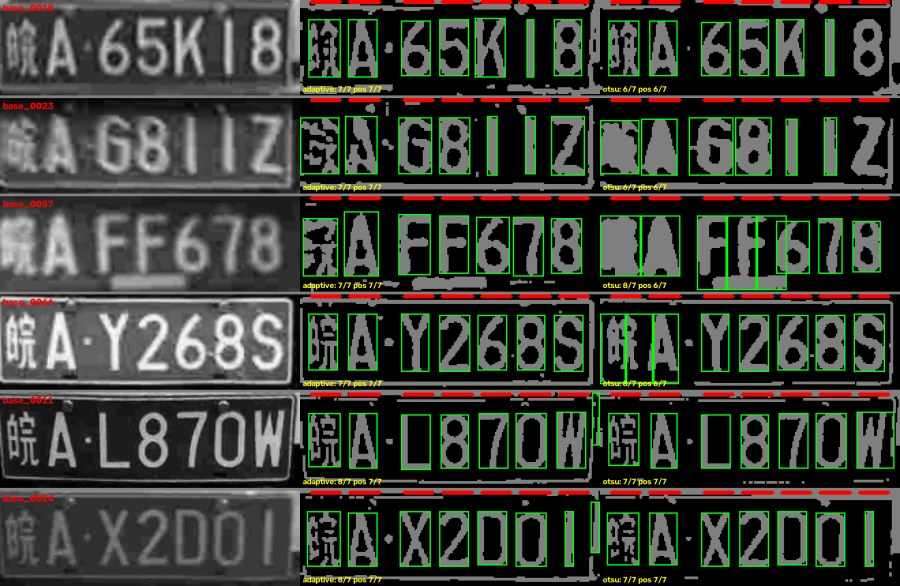
\includegraphics[width=0.78\textwidth]{figures/e5_binarize.jpg}
\caption[Ví dụ Otsu và adaptive]{Ví dụ trên tune: ảnh biển (trái), adaptive (giữa), Otsu (phải); hộp xanh lá là kết quả \code{cca}, vạch đỏ phía trên là khuôn 7 vị trí. Otsu làm dính ký tự Hán với ``A'' và dính ``FF'' ở biển mờ hoặc chói (\code{base\_0023}, \code{base\_0057}); adaptive giữ nét rời nhưng sinh hộp thừa ở mép viền (\code{base\_0011}, \code{base\_0024}). Hình chụp ở giai đoạn tune (code trước bản chốt tách ký tự), chỉ để minh họa.}
\label{fig:e5}
\end{figure}

\textbf{Nhận xét.}
\begin{itemize}
  \item Trên test Otsu cao hơn: \code{all\_correct} 0.563 so với 0.509. Tính theo cặp ảnh, Otsu đúng hết mà adaptive sai ở 90 biển, ngược lại 65 biển (sign test hai phía, $p\approx 0.054$): chênh lệch ở ngưỡng có ý nghĩa nhưng không ổn định, vì trên tune adaptive lại nhỉnh hơn. Kết luận thận trọng là hai cách tương đương, Otsu (cấu hình mặc định) không thua.
  \item Adaptive trúng vị trí nhiều hơn (\code{pos0} 0.859 so với 0.805, \code{pos1\textendash 6} 0.875 so với 0.815) nhưng sai số hộp nhiều hơn. Phân bố số hộp trên crop \code{gt} cho thấy hai kiểu lỗi ngược nhau: với Otsu, 148 biển có $\le 6$ hộp (thiếu, do dính) và 34 biển có $\ge 8$ hộp; với adaptive là 115 và 85. Tức Otsu hay làm \emph{dính} ký tự, adaptive hay sinh hộp \emph{thừa} từ mép viền và vệt nhiễu (Hình~\ref{fig:e5}).
  \item Theo nhóm: adaptive tốt hơn ở \code{challenge} và \code{blur} (theo \code{count\_match}), nơi độ sáng không đều làm một ngưỡng toàn cục thất bại; Otsu tốt hơn rõ ở \code{db} (0.393 so với 0.250), vì biển tối có tương phản thấp hơn $C=7$ nên adaptive làm vỡ nét chữ. Mỗi nhóm chỉ 28 ảnh nên các chênh lệch này chỉ mang tính gợi ý.
  \item Cả hai cách đều rất nhanh (dưới 1.1 ms/biển gồm cả tách ký tự), không ảnh hưởng tới thời gian toàn pipeline.
\end{itemize}

\section{Tách ký tự: CCA và projection (E6)}
\label{sec:e6}

\subsection{Quá trình tinh chỉnh trên tune}
\label{sec:segtune}

Bảng~\ref{tab:segtune} tóm tắt các lần sửa, tất cả đo trên tune ($n=198$), crop \code{gt} + quad. Mỗi bước đều xuất phát từ việc đọc ảnh lỗi chứ không phải quét lưới tham số.

\begin{table}[htbp]
\centering
\caption[Tinh chỉnh tách ký tự trên tune]{Tinh chỉnh tách ký tự trên tune ($n=198$, crop \code{gt} + quad), \code{all\_correct}. Nguồn: sổ thí nghiệm, mục Tách ký tự.}
\label{tab:segtune}
\small
\rowcolors{2}{white}{tablerowalt}
\arrayrulecolor{tableheader}
\begin{tabularx}{\textwidth}{YCCCC}
\hline
\rowcolor{tableheader} \tblhd{Phiên bản} & \tblhd{Otsu + CCA} & \tblhd{Otsu + proj.} & \tblhd{adapt. + CCA} & \tblhd{adapt. + proj.} \\
\hline
Bản đầu (xóa mọi khối rộng $>30\%$, metric IoU) & 0.338 & -- & -- & -- \\
Giữ khối đặc rộng để cắt & 0.364 & -- & 0.369 & 0.369 \\
Luật tâm cho hộp hẹp, tỉ lệ min 0.10 & 0.515 & 0.566 & 0.515 & 0.490 \\
\textbf{Bản chốt} & 0.540 & \textbf{0.596} & 0.566 & 0.530 \\
\hline
\end{tabularx}
\end{table}

Ba thay đổi của bản chốt: (i) ngưỡng ``mảnh hẹp'' dùng hằng số riêng 0.15 thay vì dùng chung cận dưới tỉ lệ ký tự (đã hạ xuống 0.10 cho chữ số ``1''), nếu không các mảnh ký tự Hán có tỉ lệ 0.10--0.15 không còn được gộp; (ii) số phần cắt tính có khe $g$ thay vì $\operatorname{round}(w/w_{\mathrm{med}})$; (iii) chỉ bỏ mảnh dẹt sau khi đã gộp mảnh chồng, để nét ngang của ký tự Hán được gộp vào ký tự trước. Không tổ hợp nào giảm \code{all\_correct}; với adaptive + CCA là 7 biển đúng thêm, 1 biển mất. Vì các hằng số này được chọn trên chính tune, số tune hơi lạc quan. Thay đổi có tác dụng lớn nhất trong quá trình tinh chỉnh là sửa độ đo cho chữ số ``1'' (tune: 0.364 $\to$ 0.515); tiếp theo là các sửa của bản chốt và cắt tại thung lũng của projection.

Theo quy tắc chọn trên tune, tổ hợp tốt nhất là \textbf{Otsu + projection} (0.596). Tập test khẳng định lựa chọn này (bên dưới). Tuy vậy, config mặc định vẫn đặt \code{segment.method: cca} và triage ở mục~\ref{sec:triage} dùng CCA; việc đổi cấu hình mặc định sang projection chưa được thực hiện.

\subsection{Kết quả trên test}
\label{sec:e6test}

Bảng~\ref{tab:e6} cho \code{all\_correct} của hai bộ tách với hai nguồn crop: \code{gt} (quad thật, đo riêng bộ tách) và \code{pred} (quad dự đoán của top-1 \code{edge\_svm} + bilateral trên mọi ảnh, định vị sai tính là hỏng). Nhị phân hóa theo config (Otsu).

\begin{table}[htbp]
\centering
\caption[E6: CCA và projection (test)]{E6: \code{all\_correct} của CCA và projection, tập test, nhị phân Otsu, crop quad. Hai dòng cuối là các độ đo khác của dòng ALL. Nguồn: \code{e6\_segmentation.csv}.}
\label{tab:e6}
\small
\rowcolors{2}{white}{tablerowalt}
\arrayrulecolor{tableheader}
\begin{tabularx}{\textwidth}{lcCCCC}
\hline
\rowcolor{tableheader} \tblhd{Nhóm} & \tblhd{$n$} & \tblhd{CCA gt} & \tblhd{proj. gt} & \tblhd{CCA pred} & \tblhd{proj. pred} \\
\hline
base & 350 & 0.666 & \textbf{0.749} & 0.243 & \textbf{0.277} \\
blur & 28 & 0.143 & \textbf{0.214} & 0.000 & \textbf{0.071} \\
challenge & 28 & 0.143 & \textbf{0.214} & \textbf{0.071} & 0.000 \\
db & 28 & \textbf{0.393} & 0.250 & \textbf{0.107} & 0.071 \\
tilt & 28 & 0.286 & 0.286 & 0.000 & 0.000 \\
\hline
ALL & 462 & 0.563 & \textbf{0.626} & 0.195 & \textbf{0.219} \\
\hline
ALL, \code{count\_match} & 462 & 0.606 & 0.680 & 0.400 & 0.422 \\
ALL, \code{pos1\textendash 6} & 462 & 0.815 & 0.864 & 0.518 & 0.477 \\
\hline
\end{tabularx}
\end{table}

\begin{figure}[htbp]
\centering
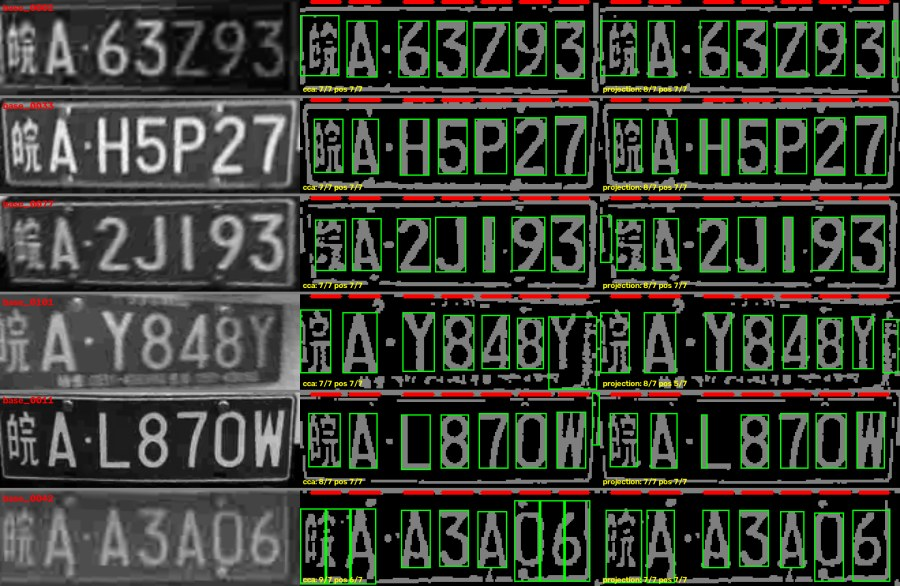
\includegraphics[width=0.78\textwidth]{figures/e6_segment.jpg}
\caption[Ví dụ CCA và projection]{Ví dụ trên tune: ảnh biển (trái), CCA (giữa), projection (phải), cùng ảnh nhị phân adaptive. CCA cắt đều khối ``06'' dính chấm nhiễu thành 3 hộp (\code{base\_0042}, 9/7); projection không bị vì chấm nhiễu không đủ 10\% chiều cao cột, nhưng hay sinh hộp thừa ở mép trái/phải (\code{base\_0002}, \code{base\_0077}). Hình chụp ở giai đoạn tune (code trước bản chốt tách ký tự), chỉ để minh họa.}
\label{fig:e6}
\end{figure}

\textbf{Nhận xét.}
\begin{itemize}
  \item \textbf{Projection tốt hơn CCA trên crop \code{gt}}: 0.626 so với 0.563. Tính theo cặp ảnh, projection đúng hết mà CCA sai ở 47 biển, ngược lại 18 biển (sign test, $p<0.001$). Kết quả cùng chiều với tune (0.596 so với 0.540), nên đây là khác biệt ổn định. Lợi thế đến chủ yếu từ \code{count\_match} (0.680 so với 0.606): cắt tại thung lũng của profile cột chính xác hơn cắt đều, và các vệt nhiễu mảnh không đủ cao để thành cột chữ. Phân bố số hộp xác nhận điều này: số biển có $\le 6$ hộp giảm từ 148 (CCA) xuống 110 (projection), còn số biển có $\ge 8$ hộp gần như không đổi (34 và 38).
  \item Projection thua khi ký tự có cột giữa thưa: chữ ``H'' chỉ có vạch ngang mảnh ở giữa nên bị cắt thành hai nét đứng hẹp rồi bị loại; phần móc dưới của ``J'' làm hộp lệch. CCA tốt hơn ở \code{db} (0.393 so với 0.250), nơi ảnh nhị phân của biển tối có nhiều vệt dọc nối vào ký tự.
  \item \textbf{Khoảng cách \code{gt} $\to$ \code{pred} rất lớn} (0.626 $\to$ 0.219 với projection): phần lớn lỗi của toàn pipeline nằm trước bước tách. Ngoài khoảng 25\% ảnh định vị sai, quad dự đoán lệch trung bình 16 px (E4) cũng làm hỏng crop. Triage (mục~\ref{sec:triage}) cho con số tương ứng: trong 123 ảnh lỗi \code{segment\_count}, 64 ảnh tách đúng nếu crop bằng quad thật.
  \item Lỗi do chính bộ tách (đúng cả khi crop \code{gt}) tập trung ở hai chỗ: ký tự Hán dính với chữ ``A'' (thường ra 6 hộp), và mảnh viền hoặc ốc vít ở mép được giữ lại thành hộp thứ 8. Các nhóm khó gần như không có biển đúng hết ngay cả khi crop \code{gt} (0.143--0.393), do ảnh nhị phân đã hỏng từ trước (mờ thành khối đặc, tối thì vỡ nét).
  \item Thời gian tách rất nhỏ: khoảng 0.8 ms/biển với CCA và 1.5 ms/biển với projection (gồm cả nhị phân hóa).
\end{itemize}

\subsection{Đánh giá theo hộp ký tự gán tay}
\label{sec:charbox}

Độ đo theo vị trí khuôn không cho biết hộp có ôm sát ký tự hay không. Để bổ sung, nhóm gán tay hộp ký tự cho 30 biển test cố định (22 biển \code{base} và 2 biển mỗi nhóm khó, chọn bằng seed trong config, gán theo cùng một quy ước: mỗi ký tự một hộp ôm sát nét chữ, ký tự Hán là một hộp, không gán dấu chấm, viền, ốc vít). Precision, recall, F1 tính theo hộp với ngưỡng IoU 0.5, ghép một-một, cộng dồn TP/FP/FN trên mọi biển (Bảng~\ref{tab:charprf}).

\begin{table}[htbp]
\centering
\caption[P/R/F1 theo hộp ký tự gán tay (test)]{P/R/F1 theo hộp ký tự gán tay, 30 biển test (210 hộp), crop \code{gt} + quad, nhị phân Otsu. Mỗi nhóm khó chỉ 2 biển (14 hộp). Nguồn: \code{e6\_segmentation.csv}.}
\label{tab:charprf}
\small
\rowcolors{2}{white}{tablerowalt}
\arrayrulecolor{tableheader}
\begin{tabularx}{\textwidth}{lcCCCC}
\hline
\rowcolor{tableheader} \tblhd{Nhóm} & \tblhd{Số biển} & \tblhd{F1 CCA} & \tblhd{F1 proj.} & \tblhd{R CCA} & \tblhd{R proj.} \\
\hline
base & 22 & 0.950 & \textbf{0.977} & 0.935 & \textbf{0.961} \\
blur & 2 & \textbf{0.211} & 0.200 & 0.143 & 0.143 \\
challenge & 2 & \textbf{0.421} & 0.316 & \textbf{0.286} & 0.214 \\
db & 2 & 0.929 & \textbf{0.963} & 0.929 & 0.929 \\
tilt & 2 & 0.783 & \textbf{0.833} & 0.643 & \textbf{0.714} \\
\hline
ALL & 30 & 0.878 & \textbf{0.896} & 0.819 & \textbf{0.838} \\
\hline
\end{tabularx}
\end{table}

Trên cả 30 biển, CCA đạt $P=0.945$, $R=0.819$, $F_1=0.878$; projection đạt $P=0.962$, $R=0.838$, $F_1=0.896$, cùng chiều với \code{all\_correct} ở Bảng~\ref{tab:e6}. Với 22 biển \code{base}, F1 của projection là 0.977. Precision của cả hai cao hơn recall rõ rệt: khi đã sinh ra hộp thì hộp thường ôm đúng ký tự, lỗi chủ yếu là \emph{thiếu} hộp (ký tự dính nhau hoặc bị lọc mất), khớp với nhận xét ở trên. Recall thấp nhất ở \code{blur} và \code{challenge} (0.14--0.29), nơi ảnh nhị phân đã hỏng từ trước. Vì mỗi nhóm khó chỉ có 2 biển, các số theo nhóm khó chỉ để tham khảo.

\section{Thời gian chạy từng bước (E7)}
\label{sec:e7}

E7 đo thời gian từng bước của pipeline đầy đủ trên test (Bảng~\ref{tab:e7}), một tiến trình, ms/ảnh.

\begin{table}[htbp]
\centering
\caption[E7: thời gian từng bước (test, ALL)]{E7: thời gian từng bước, tập test, dòng ALL (ms/ảnh). Nguồn: \code{e7\_runtime.csv}. Bước ``Sobel, morph, lọc, NMS'' được ước lượng bằng hiệu thời gian \code{localize\_edge} trừ thời gian tiền xử lý đo riêng. 30 ảnh không có ứng viên nên các bước sau định vị chỉ có $n=432$.}
\label{tab:e7}
\small
\rowcolors{2}{white}{tablerowalt}
\begin{tabular}{lrrr}
\toprule
\rowcolor{tableheader} \tblhd{Bước} & \tblhd{$n$} & \tblhd{tb (ms)} & \tblhd{p95 (ms)} \\
\midrule
tiền xử lý (resize, xám, CLAHE, lọc) & 462 & 69.79 & 134.32 \\
Sobel, morph đa tỉ lệ, lọc, NMS (ước lượng) & 462 & 63.50 & 149.30 \\
HOG + SVM & 462 & 4.77 & 10.77 \\
ước lượng quad & 432 & 0.97 & 2.20 \\
warp 220$\times$70 & 432 & 0.34 & 0.59 \\
nhị phân hóa (B) & 432 & 0.10 & 0.18 \\
tách ký tự (B) & 432 & 0.43 & 0.76 \\
\midrule
\textbf{tổng (không SVM)} & 462 & 135.01 & 247.69 \\
\textbf{tổng} & 462 & 139.79 & 262.16 \\
\bottomrule
\end{tabular}
\end{table}


Tổng thời gian trung bình là 139.8 ms/ảnh (p95 262.2 ms). Định vị chiếm gần như toàn bộ: tiền xử lý khoảng 50\% (69.8 ms, phần lớn là bilateral đường kính 11 trên ảnh 800 px), Sobel cùng morph đa tỉ lệ khoảng 45\% (63.5 ms), SVM khoảng 3\% (4.8 ms). Các bước nắn, nhị phân hóa và tách ký tự cộng lại chỉ 1.8 ms. Theo nhóm, \code{tilt} chậm nhất (208.4 ms) và \code{challenge} nhanh nhất (88.5 ms; \code{db} 92.6 ms). Số tuyệt đối trong lần đo ghi trong sổ thí nghiệm cao hơn nhiều (416 ms/ảnh) vì máy khi đó đang chạy nhiều tiến trình; tỉ lệ giữa các bước cũng dịch theo tải máy (tiền xử lý 44\% $\to$ 50\%, Sobel cùng morph 51\% $\to$ 45\%, SVM 3.3\% $\to$ 3.4\%), nên chỉ xem tỉ lệ là gần đúng. Nếu cần số tuyệt đối cho kết luận về tốc độ thì nên đo lại trên máy riêng.

\section{Ảnh biển số Việt Nam, đánh giá định tính (E8)}
\label{sec:e8}

\textbf{Mục tiêu.} E8 chạy pipeline tốt nhất (định vị \code{edge\_svm} + bilateral, nắn quad về $220\times 70$, Otsu, projection) trên ảnh biển số Việt Nam (split \code{qual}) và xem kết quả bằng mắt, để biết pipeline xây trên CCPD tổng quát hóa tới đâu. Bộ ảnh gồm 187 ảnh (75 + 64 ảnh Kaggle và 48 ảnh lấy bằng tìm kiếm Brave, xem mục~\ref{sec:data}); mới có bbox cho 139 ảnh Kaggle nên E8 chạy trên 139 ảnh này, 48 ảnh còn lại chờ gán bbox. Mỗi ảnh chạy hai lần: trên crop quanh ứng viên top-1 của bước định vị (\code{pred}) và trên crop theo bbox thật (\code{gt}). Crop theo bbox là hình chữ nhật chứ không phải nắn quad, nên hai cách crop không hoàn toàn tương đương. Kết quả từng ảnh ghi ở \code{results/tables/e8\_vn.csv}; E8 không có độ đo chính thức. Hai cột ``đạt'' dưới đây chỉ là kiểm tra thô, không phải độ đo: \emph{định vị đạt} khi ứng viên top-1 trùng bbox thật (IoU đủ ngưỡng), \emph{tách đạt} khi bộ tách cho 7--10 hộp và số dòng khớp nhãn.

\textbf{Kết quả.} Trên 139 ảnh, định vị đạt 40 ảnh (29\%), tách đạt 33 ảnh trên crop \code{gt} và 22 ảnh trên crop \code{pred}. Số theo nhóm (chỉ để minh họa, nhóm nhỏ và không cân bằng):
\begin{itemize}
  \item \textbf{Số dòng.} Biển một dòng ($n=44$): định vị đạt 28 (0.64), tách đạt 30 (0.68) trên crop \code{gt} và 22 (0.50) trên crop \code{pred}. Biển hai dòng ($n=95$): định vị đạt 12 (0.13), tách đạt 3 trên crop \code{gt} và 0 trên crop \code{pred}.
  \item \textbf{Loại xe.} Ô tô ($n=66$): định vị đạt 34 (0.52). Xe máy ($n=61$): 2 (0.03). Xe tải ($n=12$): 4 (0.33). Cả 61 biển xe máy đều có hai dòng.
  \item \textbf{Màu biển.} Biển trắng ($n=131$): định vị đạt 40 (0.31); biển vàng ($n=6$): 0; biển xanh và biển đỏ mỗi loại 1 ảnh, đều không định vị đạt. Với $n$ nhỏ như vậy các số này chỉ mang tính giai thoại.
\end{itemize}

\begin{figure}[htbp]
\centering
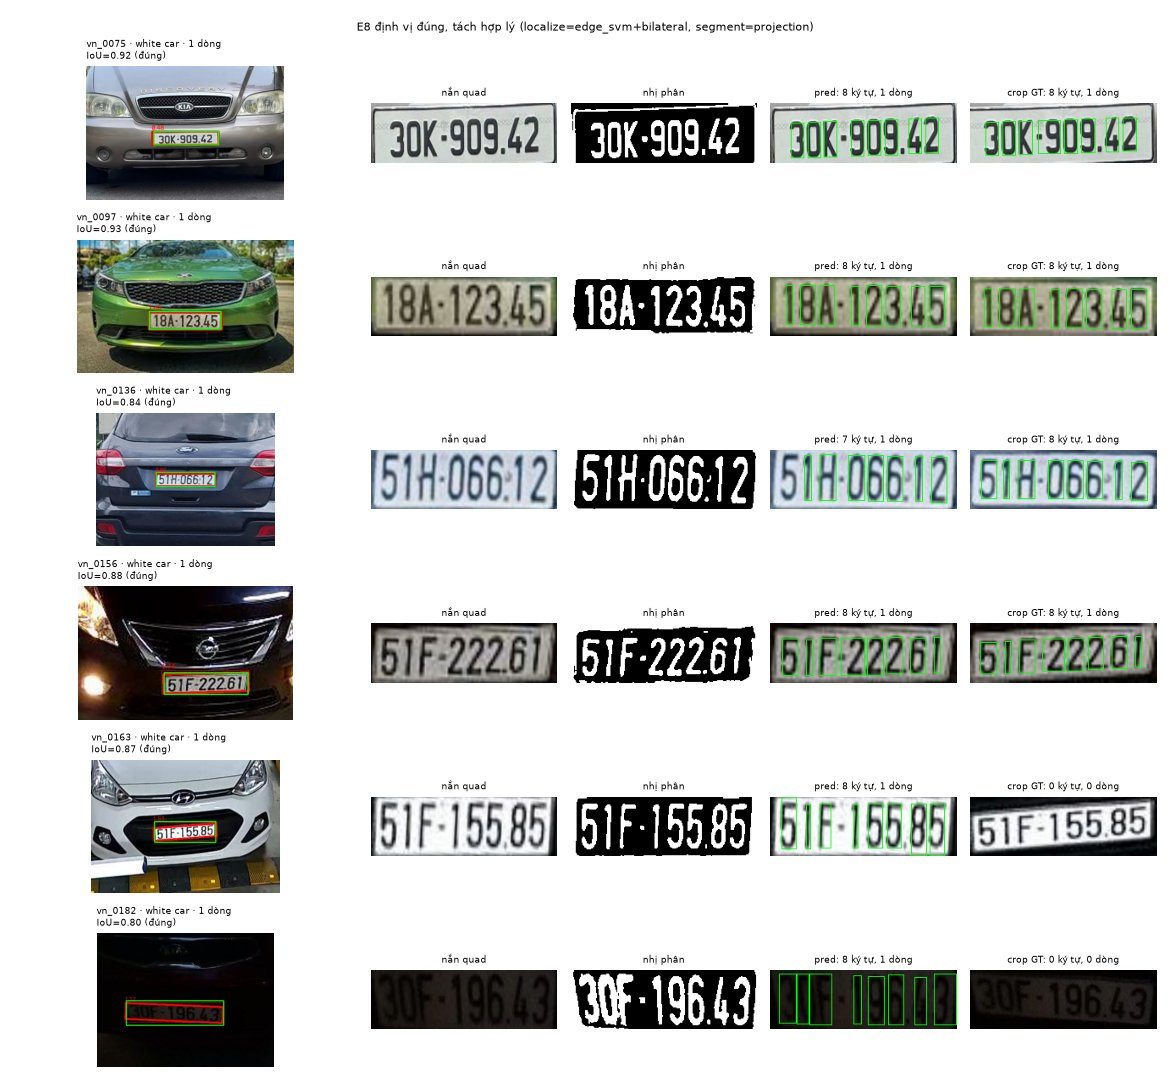
\includegraphics[width=0.88\textwidth]{figures/vn_success.jpg}
\caption[E8: biển một dòng định vị đúng]{E8, biển một dòng định vị đúng (hộp xanh lá: bbox thật, đỏ: ứng viên top-1). Mỗi hàng, từ trái sang phải: ảnh với hai hộp, biển sau nắn quad, ảnh nhị phân, crop \code{pred} và crop \code{gt} kèm hộp ký tự. Bốn hàng đầu tách tốt. Ở \code{vn\_0163} crop \code{gt} cho 0 ký tự dù biển rõ; ở \code{vn\_0182} (biển tối) các hộp ký tự lệch dù định vị đúng.}
\label{fig:e8-ok}
\end{figure}

\begin{figure}[htbp]
\centering
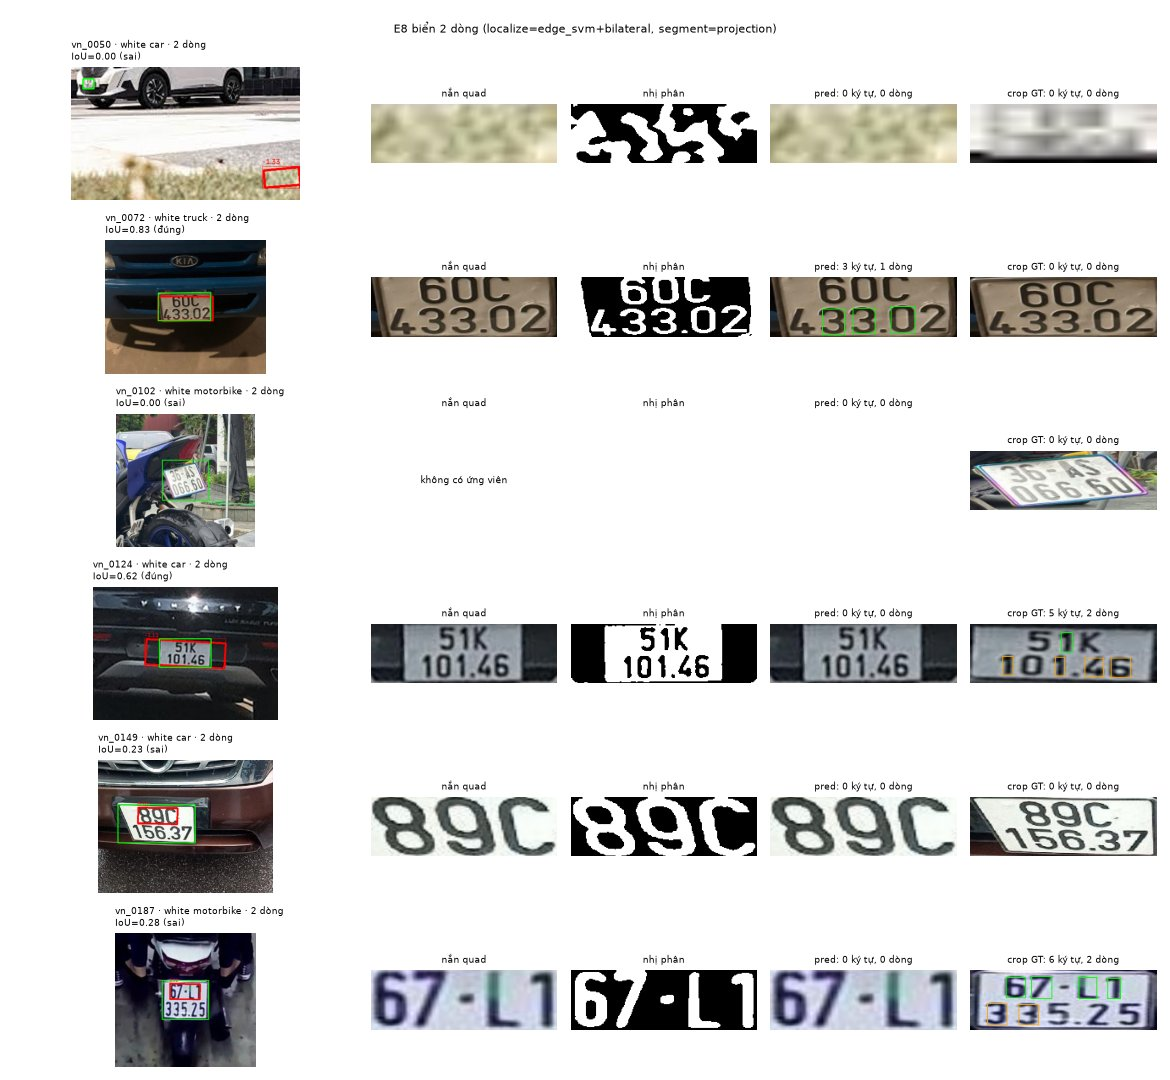
\includegraphics[width=0.88\textwidth]{figures/vn_two_line.jpg}
\caption[E8: biển hai dòng]{E8, biển hai dòng. Dù ứng viên top-1 đúng (\code{vn\_0072}, \code{vn\_0124}), bộ tách chỉ ra 3 hộp hoặc không ra hộp nào; \code{vn\_0102} không có ứng viên; ở \code{vn\_0149} ứng viên chỉ phủ dòng trên của biển.}
\label{fig:e8-two}
\end{figure}

\begin{figure}[htbp]
\centering
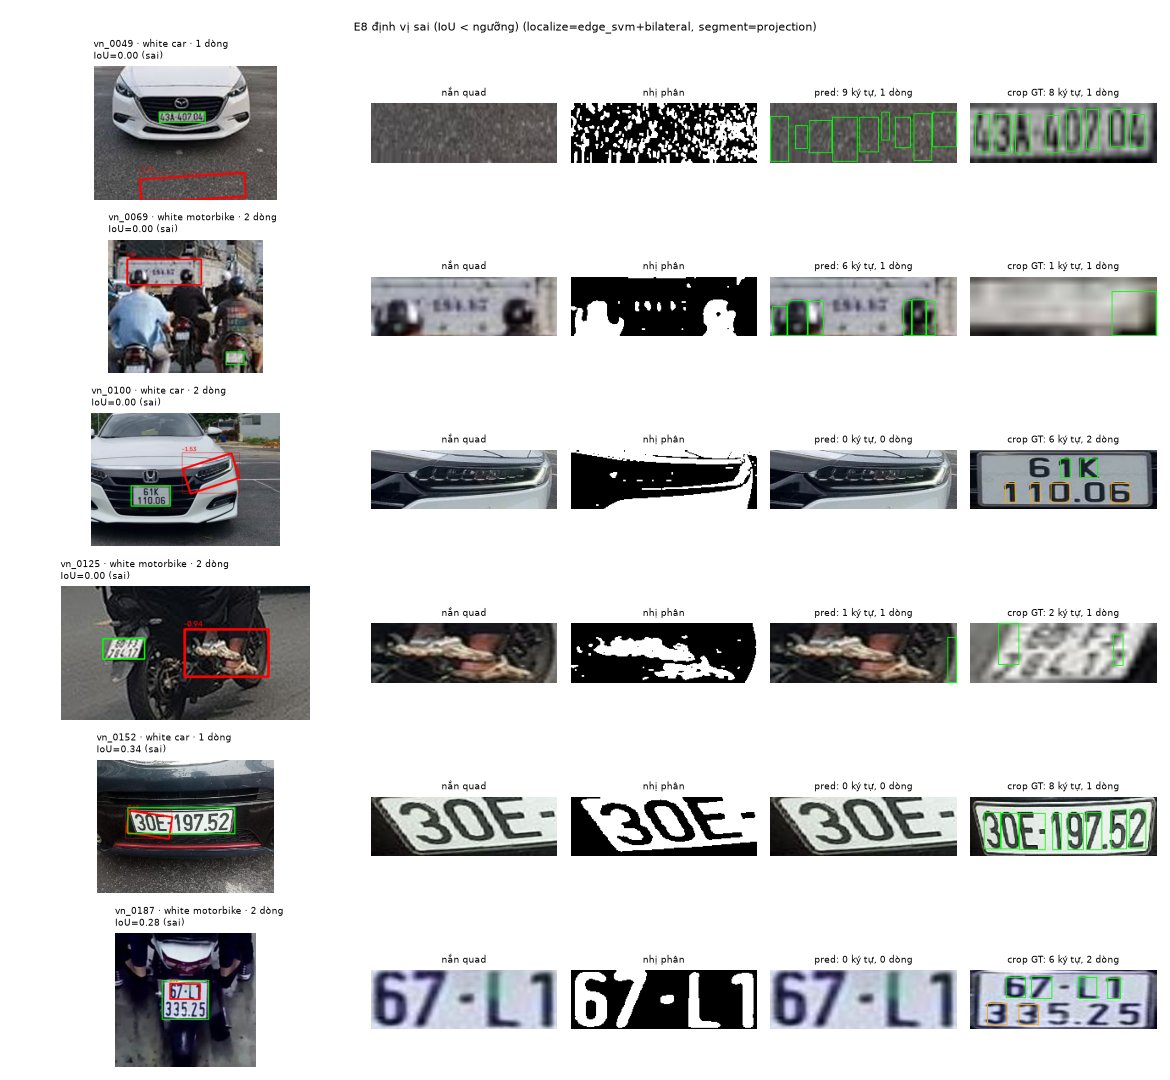
\includegraphics[width=0.88\textwidth]{figures/vn_loc_fail.jpg}
\caption[E8: định vị sai]{E8, định vị sai (IoU dưới ngưỡng). Ứng viên top-1 rơi vào mặt đường, đèn xe, chân người, vùng chữ/biển khác trong ảnh đông xe (\code{vn\_0069}); ở \code{vn\_0152} và \code{vn\_0187} hộp chỉ phủ một phần biển.}
\label{fig:e8-loc}
\end{figure}

\textbf{Nhận xét.}
\begin{itemize}
  \item \textbf{Định vị là chỗ hỏng chính.} Chỉ 40/139 ảnh có ứng viên top-1 đạt. Trong sáu ví dụ ở Hình~\ref{fig:e8-loc}, các hộp sai nằm trên vùng nền nhiều cạnh (mặt đường, đèn, chân, vùng chữ/biển khác trong ảnh đông xe) hoặc chỉ phủ một phần biển, nên nắn quad sau đó cũng cắt thiếu. Biển xe máy hai dòng gần như luôn hỏng ở bước này (2/61), một số ảnh không có ứng viên nào.
  \item \textbf{Biển ô tô một dòng nền trắng chạy khá tốt} (Hình~\ref{fig:e8-ok}): ký tự được tách thành 7--9 hộp, kể cả dấu chấm và dấu gạch, không cần khuôn 7 vị trí.
  \item \textbf{Biển hai dòng tách sai ngay cả khi có hộp tốt:} chỉ 3/95 ảnh đạt trên crop \code{gt} (Hình~\ref{fig:e8-two}). Một nguyên nhân hợp lý là biển gần vuông bị nắn thành $220\times 70$ nên méo, và \code{split\_lines} được chỉnh trên CCPD; chúng tôi không có thí nghiệm cô lập (ví dụ nắn theo tỉ lệ riêng) để khẳng định.
  \item \textbf{Crop theo bbox khác nắn quad:} ở 20 ảnh, crop \code{gt} cho 0 ký tự trong khi crop \code{pred} cho ít nhất một hộp (ví dụ \code{vn\_0163}, \code{vn\_0182} ở Hình~\ref{fig:e8-ok}), nên số ``tách đạt trên \code{gt}'' không phải trần của bộ tách.
  \item \textbf{Biển màu và ảnh ban đêm.} Biển vàng, xanh, đỏ đều không được định vị đạt, phù hợp với dự đoán rằng SVM chỉ học trên biển xanh của CCPD, nhưng $n$ quá nhỏ để kết luận. Ảnh ban đêm có kết quả lẫn lộn (định vị đạt 17/39 ảnh có thẻ \code{night}, so với 23/100 ảnh còn lại; tách đạt trên crop \code{gt} 9/39 so với 24/100); chúng tôi chưa tìm hiểu nguyên nhân.
\end{itemize}

\textbf{Đối chiếu với dự đoán từ thiết kế.} Trước khi chạy, các phần trên gợi ý ba chỗ khó; kết quả E8 cho thấy:
\begin{itemize}
  \item \textbf{Màu nền.} Dự đoán rằng SVM học trên biển xanh sẽ khó với biển trắng và vàng. Phù hợp một phần: biển trắng ô tô một dòng vẫn định vị được khá nhiều, còn biển vàng (6 ảnh) không ảnh nào đạt. Bước nhị phân hóa tự đoán cực tính nên chữ vẫn ra trắng trên nền đen khi biển được định vị đúng (Hình~\ref{fig:e8-ok}).
  \item \textbf{Biển hai dòng.} Dự đoán đúng, và nặng hơn dự kiến: \code{split\_lines} (trước đây chỉ kiểm bằng ảnh giả) gần như không cho kết quả đạt trên ảnh thật, và định vị cũng kém hơn nhiều so với biển một dòng.
  \item \textbf{Số ký tự và khuôn.} Đúng như dự đoán, khuôn 7 vị trí không dùng được; E8 chỉ kiểm bằng mắt và đếm hộp thô, không đo độ chính xác.
\end{itemize}
Tóm lại, pipeline xây trên CCPD chạy được với biển ô tô một dòng nền trắng nhưng không dùng trực tiếp được cho biển hai dòng và biển xe máy. Cần định vị riêng cho biển xe máy và nắn theo tỉ lệ hai dòng trước khi đánh giá bước tách. Đây là một lần chạy trên 139 ảnh Kaggle không cân bằng (95 biển hai dòng, 61 biển xe máy), không phải ước lượng cho biển Việt Nam nói chung.
